\renewcommand{\imagewidth}{0.25\linewidth}
\renewcommand{\smallimagewidth}{0.12\linewidth}
\newcommand{\offset}{0.8pt}
\begin{figure}[t]
  \centering
  \begin{subfigure}[b]{\linewidth}
    \centering
    \resizebox{\linewidth}{!}{
      \begin{tikzpicture}[
          >=stealth',
          overlay/.style={
              anchor=north west,
              draw=black,
              rectangle,
              line width=\offset,
              outer sep=0,
              inner sep=0,
            },
          every node/.style={inner sep=0,outer sep=0}
        ]
        \matrix[matrix of nodes, column sep=-1pt, row sep=0, ampersand replacement=\&] (datarep) {
          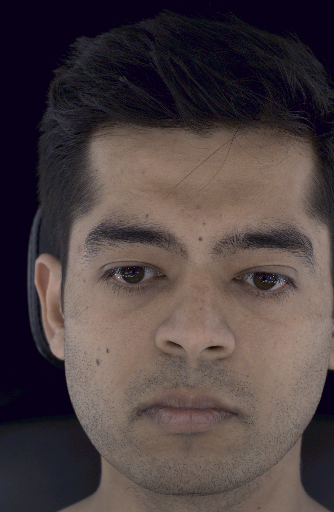
\includegraphics[width=\imagewidth,trim={1.2cm 0 0 0},clip]{assets/\blendfieldsdirname/data/gt/002757580_28_0.png} \&
          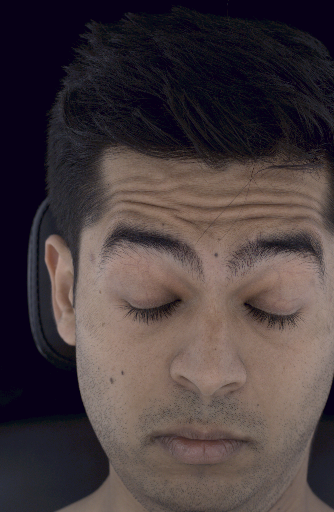
\includegraphics[width=\imagewidth,trim={1.2cm 0 0 0},clip]{assets/\blendfieldsdirname/data/gt/002757580_28_1.png} \&
          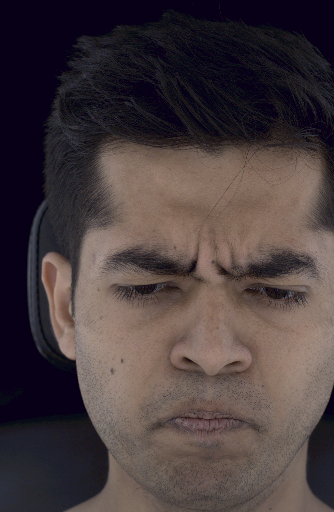
\includegraphics[width=\imagewidth,trim={1.2cm 0 0 0},clip]{assets/\blendfieldsdirname/data/gt/002757580_28_3.png} \&
          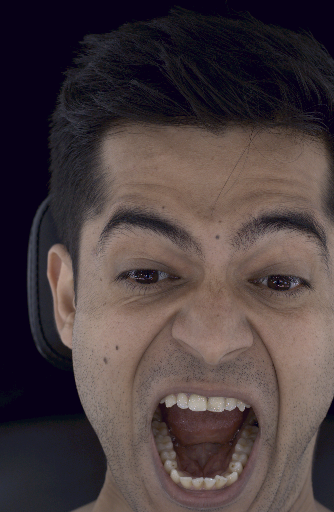
\includegraphics[width=\imagewidth,trim={1.2cm 0 0 0},clip]{assets/\blendfieldsdirname/data/gt/002757580_28_4.png} \\ % \&
          % \includegraphics[width=\imagewidth]{assets/data/gt/002757580_28_7.png}
          % \\
        };
        \node[below right=\offset and \offset of datarep-1-1.north west, overlay]{
          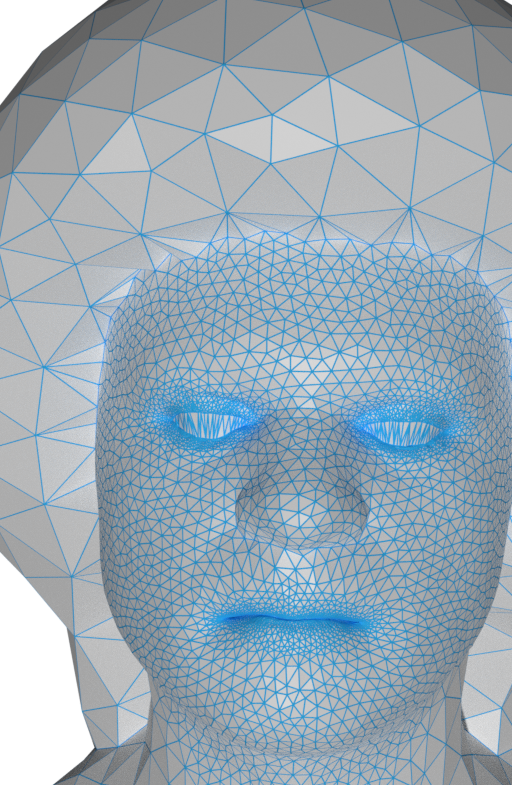
\includegraphics[width=\smallimagewidth]{assets/\blendfieldsdirname/data/wireframes/mesh_frame_0.png}
        };
        \node[below right=\offset and \offset of datarep-1-2.north west, overlay]{
          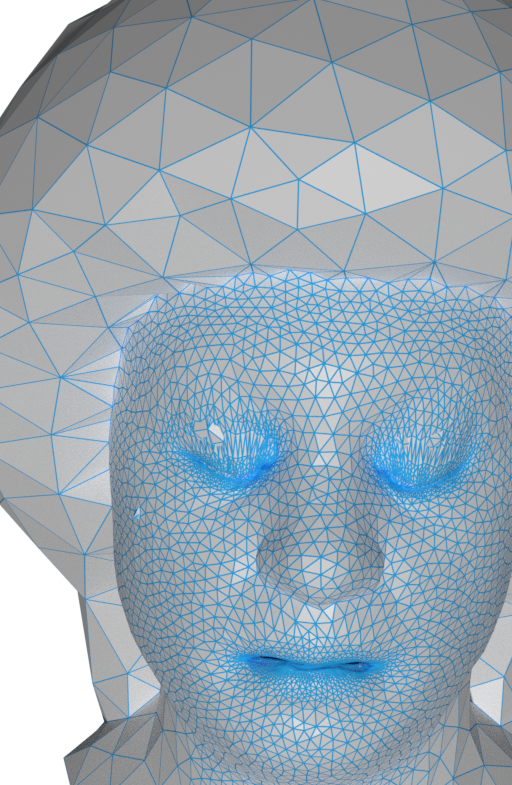
\includegraphics[width=\smallimagewidth]{assets/\blendfieldsdirname/data/wireframes/mesh_frame_1.png}
        };
        \node[below right=\offset and \offset of datarep-1-3.north west, overlay]{
          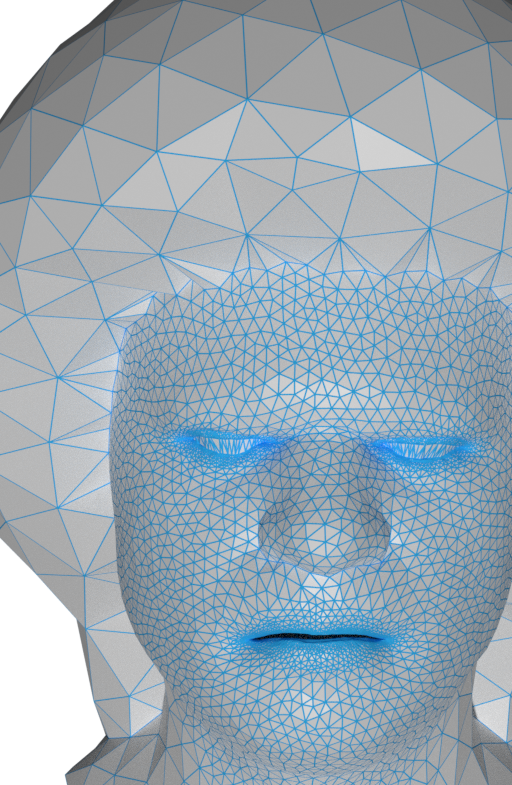
\includegraphics[width=\smallimagewidth]{assets/\blendfieldsdirname/data/wireframes/mesh_frame_3.png}
        };
        \node[below right=\offset and \offset of datarep-1-4.north west, overlay]{
          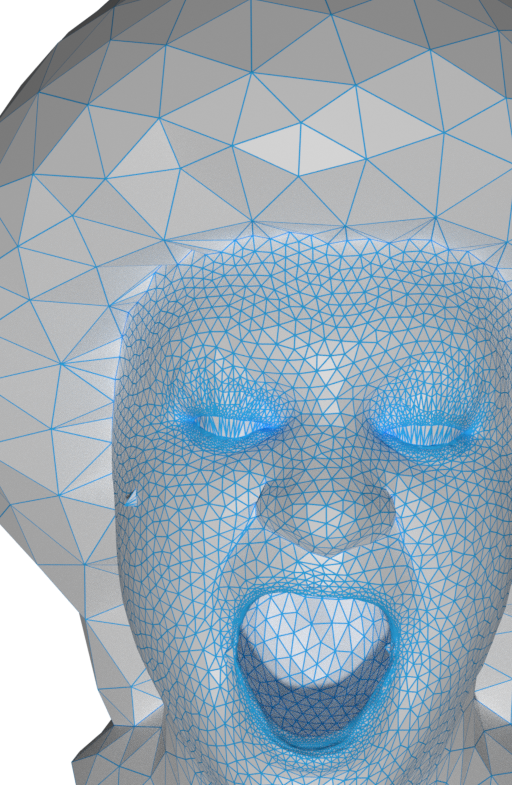
\includegraphics[width=\smallimagewidth]{assets/\blendfieldsdirname/data/wireframes/mesh_frame_4.png}
        };
        % \node[below right=\offset and \offset of datarep-1-5.north west,
        % overlay]{
        % \includegraphics[width=\smallimagewidth]{assets/data/wireframes/mesh_frame_7.png}
        % };
      \end{tikzpicture}
    }
  \end{subfigure}
  \caption{\textbf{Data} -- We represent the data as a multi-view, multi-expression images.
    For each of these images, we obtain parameters of a parametric model, such
    as FLAME \cite{li2017flame} to get: an expression vector $\expression$ and
    a tetrahedral mesh described by vertices $\meshVertices(\expression)$.
    We highlight that our approach works for any object if a rough mesh and
    its descriptor are already provided.
  }
  \label{fig:blendfields-data-representation}
\end{figure}